\chapter{Introduction}
\setcounter{page}{1}
\begin{quotation}
\noindent ``\emph{The question of whether a computer can think is no more 
	interesting than the question of whether a submarine can swim.}''
\begin{flushright}\textbf{Edsger W. Dijkstra}\end{flushright}
\end{quotation}

\vspace*{0.5cm}

\section{Context and goals}
One could trace back the birth of the machine learning idea to Alan Turing's 
seminal paper, \textit{Computing Machinery and Intelligence} 
\cite{turing1950computing}. Although the computer science context around his
work was only at its beginnings (at least compared to today), Turing already felt
the need to think of ways to transcend the fixed set of rules a computer had
to interpret and execute. As computer science grew, and as the field of
artificial intelligence went through its ebbs and flows throughout the years,
machine learning evolved from an idea to a prolific field of research, and
some of its topics saw massive application into real world domains.\\

Humans have a tendency to consider hard tasks easy and easy tasks hard.
Understanding the contents of an image should be very easy for any human
being, but it is far from it for a computer. How could a programmer write
a program or a set of rules to describe perfectly every situation that could
be presented on an image, only based on the values of its pixels? This is
of course intractable, and the whole appeal of machine learning is that it
allows us to build systems that \textit{learn} their own set of rules from
their own experience (by seeing many examples of images being
described). One only has to create a program with learnable parameters and an
algorithm that will tune the program to make it perform better with every
example it sees instead of writing a highly complex set of rules and 
instructions. The second obvious advantage of this method is that the existing
machine learning techniques to this day are very general and can solve an
enormous class of problems -- one just has to show different examples to the
learning program.\\

\subsection{Data-based methods}
The most popular and widely used machine learning algorithms and techniques
fall in the category of what could be called data-based methods. One subset
of these data-based methods is called supervised learning and 
allows, among others, to classify or to predict data. 
The goal of classification is to assign a label (or a class) to a set of 
measurements. One example of this would be
to try to categorise patients that either have or don't have some disease.

The first thing to do is to collect measurements on which we can make an
informed decision. All these measurements are put together in 
the input vector $x$, also called the \textbf{feature vector}. For our example,
it could contain measurements such as blood pressure, the 
quantity of a given substance in the patient's blood, etc.

Since we want to show our algorithm examples of people who are ill but
also of people who are not ill, we will have to associate each feature vector
with a \textbf{target vector}, also called its \textbf{ground truth} $y$ 
containing all the classes of the problem : 
being ill and not being ill. In our case, we will define $y = [1, 0]$ as
an ill patient and $y = [0, 1]$ as a healthy patient.\\

\begin{figure}
	\centering
	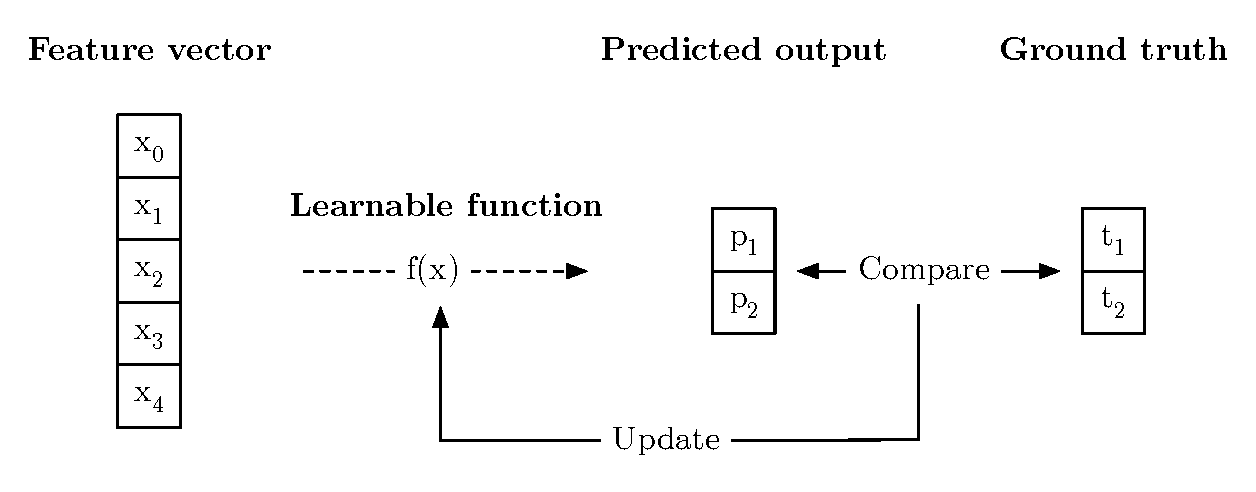
\includegraphics[width=0.8\linewidth]{fig/supervised_ml.eps}
	\caption{The supervised learning process. A feature vector and its ground
	truth $(x, t)$ are sampled from the training set. A learnable
	function computes a prediction based on the feature vector (which 
	contains measurements). We compare this prediction with the ground 
	truth and update the learnable function to minimise the error
	between the prediction and the ground truth, repeating the process
	until the function has reached a good enough accuracy.}
	\label{fig:supervised_ml}
\end{figure}

We now have have a \textbf{dataset} full of measurements $x$ associated with 
their class $y$.
If we could find a function mapping $x$ to $y$, we could then make an informed
diagnostic for a new patient with new measurements $x$ that we have never seen,
without knowing whether the patient is actually ill or not.
Supervised machine learning provides the following general process (illustrated
in Figure~\ref{fig:supervised_ml}) to find
such a function : one defines a model which has
\textit{learnable parameters} (values which impact the output of the
function) and performs \textbf{training}. The process of training is to
sample data points from a \textbf{training dataset}, containing pairs of input
vectors and output vectors. We then feed the input vector to the model, compare
the output that we get from the model (the \textbf{prediction}) 
with the output we are supposed to get (the \textbf{target}),
and tune the learnable parameters so to minimise the error between the
prediction and the target. We repeat this process, showing many samples
of the training set to the model until it reaches a good enough accuracy. Once
the function is learned, we can predict to a certain level of accuracy new 
outputs from unseen feature vectors: for example, we can compute the probability
of a new patient being ill from his or her measurements.\\

Unsupervised learning, although different from supervised learning as the
training sets usually do not have output vectors, is more about finding
structure in the dataset; but we can assume for the sake of this point that
the process is largely the same : sample data, update learnable parameters
until the model is fixed at a good enough accuracy and inference can be
performed data point by data point after training.\\

\subsection{Going further : adding interaction}
To the experienced reader, unsupervised machine learning and supervised machine
learning might sound like fancy names for statistics; and one could argue that
they are indeed. Classification and prediction are tasks that humans have
to perform on a daily basis, but they remain relatively simple. Indeed, the 
algorithms exposed above do not interact with an environment in any way and do
not perform harder tasks such as planning and developing complex strategies
to solve a given problem.\\

A subfield of machine learning that veers off slightly more
from statistics and subjectively gets closer to human-like behaviour
would be \textbf{reinforcement learning}. In this setting, we train an agent
(an entity which can perform actions, that is anything that can perceive and
act: robots, simulated software agents, ...), 
which is situated in an environment, to perform actions that will maximise
a reward given by the environment. This endeavour is orders of magnitudes more
complex to handle at first glance. One has to train an agent that has to make
assumptions about the environment it is situated in, but also set up a
potentially hierarchical strategy involving several sequences of actions.\\

This process works by letting the agent interact with the environment for many
sessions, until it figures out what actions, and what sequences of actions lead
to high rewards. This is the training process of a reinforcement learning agent.
One example of this is the CartPole problem \cite{barto-cartpole} where the
agent controls a cart on which a pole is balanced (see
Figure~\ref{fig:cartpole_illustration}). The goal is to keep the
pole balanced for as long as possible by nudging the cart left or right. The
agent receives the position of the cart, the velocity of the cart, the pole
angle and the pole velocity at tip as a state observation from the environment,
and has to push the cart either left or right. The agent will first perform
randomly, but sooner or later, it will figure out how to balance the pole.\\

\begin{figure}
	\centering
	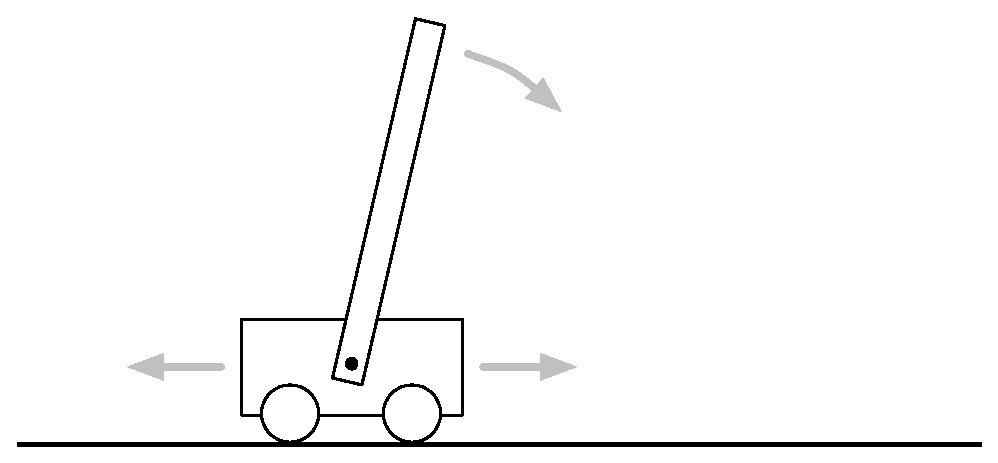
\includegraphics[width=0.8\linewidth]{fig/cartpole.eps}
	\caption{An illustration of the CartPole problem}
	\label{fig:cartpole_illustration}
\end{figure}

\subsection{One step further : learning to learn}
One common issue between all of the techniques described above is that once
training is over, the behaviour of the trained agent or model will not change
or adapt once the conditions, or some intrinsic parameters of the problem
change. If we present the CartPole agent with a pole that is twice as heavy,
or twice as long as the one it has been trained with, it will likely fail to 
balance the pole. We have taught an agent how to solve one task, but we have
not taught it to learn how to solve a task. This thesis will explore ways to 
teach an agent how to learn to solve tasks.\\

Learning to learn, as opposed to learning to solve, could open the door to a
whole new level of performance from our agents. Not only could they 
be able to generalise what they have learnt to problems that are parametrised
differently to what they have seen, but they could also learn to perform
tasks that are fundamentally different. Recent studies \cite{learningtorl,
fastrlviaslowrl} also showed their ability to perform one-shot learning in
the context of a maze : the agent shows an ability to learn the architecture
of a maze in one episode before being able to solve it from any departure point.


\section{Structure}
We will set the theoretical foundations needed to understand the methods used
in the experiments that will follow in part I. Reinforcement learning will
obviously be covered as well as artificial neural networks which serve as 
excellent learnable functions and have proven to work extremely well by
pushing the state of the art in many domains.\\

In part II, focus will be set on meta reinforcement learning : first we will
have to understand what it is and its goals are; then we will explore different
aspects and challenges related to it by inspecting how different experiments
and different parameters affect its performance.\\

Throughout part II, an analysis of the application of meta-learning to the
CartPole problem will be carried on, and discussion about why it performs
well in certain cases and why it fails in other cases will take place. We will
then propose a solution to the intrinsic problem related to the application
of meta-learning to problems similar to CartPole.


\section{Main contributions}
The main contributions of this work are twofold.

\paragraph{Meta-learning state of the art.}
A comprehensive background and state of the art are
provided to understand the goals and stakes of meta reinforcement learning.
We have implemented state of the art algorithms in meta-learning and made
their implementation public. Experiments in recent papers have been
recreated to verify and extend the results found in the literature.

\paragraph{Study of meta-learning applied to a new setting.} We apply meta-learning
to a distribution of tasks derived from the CartPole problem. We extensively
study the dynamics of meta-learning applied to a problem with a continuous
reward over long episodes, and the impact of the learning horizon (both
in terms of number of episodes the meta-learning agent is allowed to play
and the discount factor). 

We identify a critical flaw in the reward pattern provided by the CartPole
environment and propose a simple and effective strategy to counteract its
negative consequences, effectively allowing meta-learning to occur in
problems with similar continuous reward structures.
